Um die Funktionsweise beider Algorithmen zu belegen wurden beide Methoden einerseits auf ihre Robsutheit und andrerseites auf ihre Performance getestet. Im folgenden Kapitel wird zunächst das zum Testen verwendete Setup beschrieben. Anschliessend erfolgt die Auswertung der erlangten Testergebnisse. Zuletzt werden weitere Tests durchgeführt welche das System kritischen Situationen testen soll.

% ---------------------- section -----------------------
\section{Testsetup}
\label{sec:test_setup}

Bei der Durchführung der Tests befinden sich die Kameras statisch im Raum. Die zu erkennenden Hindernisse werden innerhalb und ausserhalb der zu erkennenden Reichweite platziert, wobei die Ausrichtung der Hindernisse teils zufällig, teils bewusst an kritischen Positionen erfolgt, um ein reales Anwendungsszenarien passend zu simulieren. Ein aufgenommenes Testset besteht dabei aus beiden Bildern der Kamera, der normalisierten Disparity Map sowie eine komplette Pointcloud dieser um etwaige Fehler der Algorithmen leichter erkennen zu können, sowie den geloggten Pointclouds der Hinderniserkennung. Weiterhin werden diverse Parameter gespeichert, wie die Anzahl der erkannten Hinderniselemente, sowie deren Disparitäten.\\

\noindent
Der zu erkennende Bereich wurde auf $0,2$ bis $1,5$ Meter definiert. Dies entspricht einem Szenario in welchem das System auch aufgrund der hohen Framerate der Erkennung angewendet werden kann. Eine Erweiterung dessen auf beispielsweise $2.0$ Meter wurde nicht durchgeführt, da der Algorithmus auch bei großen Entfernungen robuste Werte in der Distanzberechnung liefert \cite{hilleralhallak}.
Das dabei erreichte Sichtfeld nach der Anwendug der ROI auf die Disparity Map (siehe \ref{sec:preprocessing}) beträgt $50^{\circ}$ auf horizontaler Achse und $38^{\circ}$ vertikal. Dies ist in Abbildung (REF) visualisiert.
	% TODO sichtfeld durch disparity map & vergleich zum ursprünglichen sichtfeld

\noindent
Ein aufgenommenes Testset besteht aus jeweils 12 Testbildern. Für jede Methode wurden drei verschiedene Hindernisgrößen getestet, groß, klein und winzige Hindernisse. Anhand dieser wird ausgewertet welche minimale, maximale sowie mittlere Disparität, und daraus resultierende Distanz erkannt wird.\\

\noindent
Weitere Tests beinhalten die Erkennung winziger Hindernisse unter Veränderung der \emph{SGBM} Parameter. Dabei wird unter anderem untersucht ob beispielsweise eine verringerte Blockgröße Einfluss auf die Erkennung kleiner Bereiche nimmt. Des Weiteren wird die Zeit für die Hinderniserkennung eines Frames untersucht um eine durchschnittliche Zeit für die Erkennung sowie die daraus resultierende Framerate zu ermitteln. Dies geschieht einerseits durch die Erkennung eines Hindernisses, welches sich über das gesamte Bild ausbreitet, andererseits für nur ein Teilelement jeder Erkennungsmethode (Subimage, Samplepoint).\\
Zudem wird geprüft inwiefern die Algorithmen mit Limitierungen des \emph{SGBM} umgehen können. Dazu zählen die Erkennung bei spiegelnden, reflektierenden und durchsichtigen Flächen, sowie die Erkennung schwach texturierter Hindernisse.\\

% ---------------------- section -----------------------
\section{Evaluierung Subimage Detection}
\label{sec:evaluierung_subimage}

	 % TODO INCREASE FONTSIZE IN DIAGRAMS
    Hinsichtlich der Robustheit werden beide Algorithmen nach demselben Schema untersucht. Der in Abschnitt \ref{sec:test_setup} beschriebene Testablauf erwähnt 3 verschiedene Hindernisgrößen. Tabelle \ref{tbl:obstacle_sizes} zeigt sowohl die Maße der Hindernisse als auch deren Fläche in $cm/cm^2$ auf.
    
	\begin{table}[h]
	\centering
	\begin{tabular}{|l|c|c|c|c|}
	\hline
	Hindernis   & Radius & Länge & Breite & Fläche \\
	\hline
	Groß   		&   -    & 53.5  & 43.0   & 2300.5 \\
	\hline
	Mittel 		& 	-    & 16.0  & 14.5   & 232.0\\
	\hline
	Winzig		& 2.5	 &   -   &   -    & 19.6 \\
	\hline	
	\end{tabular}
	\label{tbl:obstacle_sizes}
	\caption{Maße der verschiedenen genutzten Hindernisse}
	\end{table}
	
	\noindent
	Während der Tests wurde für jedes aufgenommene Einzelbild die reale Distanz gemessen. Der dabei verwendete Referenzpunkt befand sich in der Mitte des zu erkennenden Hindernisses, da diese nicht zwangsläufig orthogonal zur Bildebene platziert wurden. Somit entspricht die gemessene Distanz der mittleren Distanz welche sich aus allen gefundenen Bereichen eines Bildes zusammensetzt. Während der Aufnahme sind die jeweiligen Einzelbilder der linken und rechten Kamera sowie die berechnete Disparity Map sichtbar. Weiterhin ist ein weiterer Anzeigemodus verfügbar welcher die gefundenen Hindernisse innerhalb der Tiefenkarte markiert (siehe Abbildung \ref{fig:test_viewing}). Weiterhin kann jede erstellte Hindernis-Pointcloud im Nachhinein gerendert werden um einen überblick über die Ergebnisse des Algorithmus zu erhalten.\\
	
	\begin{figure}[h]
		\centering
		\begin{tabular}{c c}
		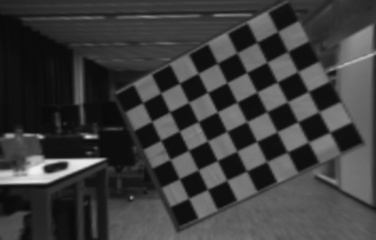
\includegraphics[width=5.0cm]{img/evaluation/test_set/_test_3_left}&
		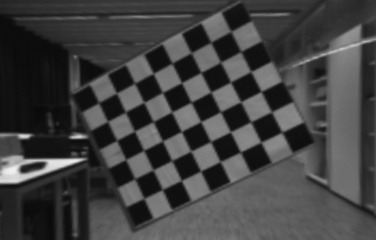
\includegraphics[width=5.0cm]{img/evaluation/test_set/_test_3_right}\\
		(a) linkes Kamerabild & (b) rechtes Kamerabild\\
		
\includegraphics[width=5.0cm]{img/evaluation/test_set/_test_3_disparity}&
	    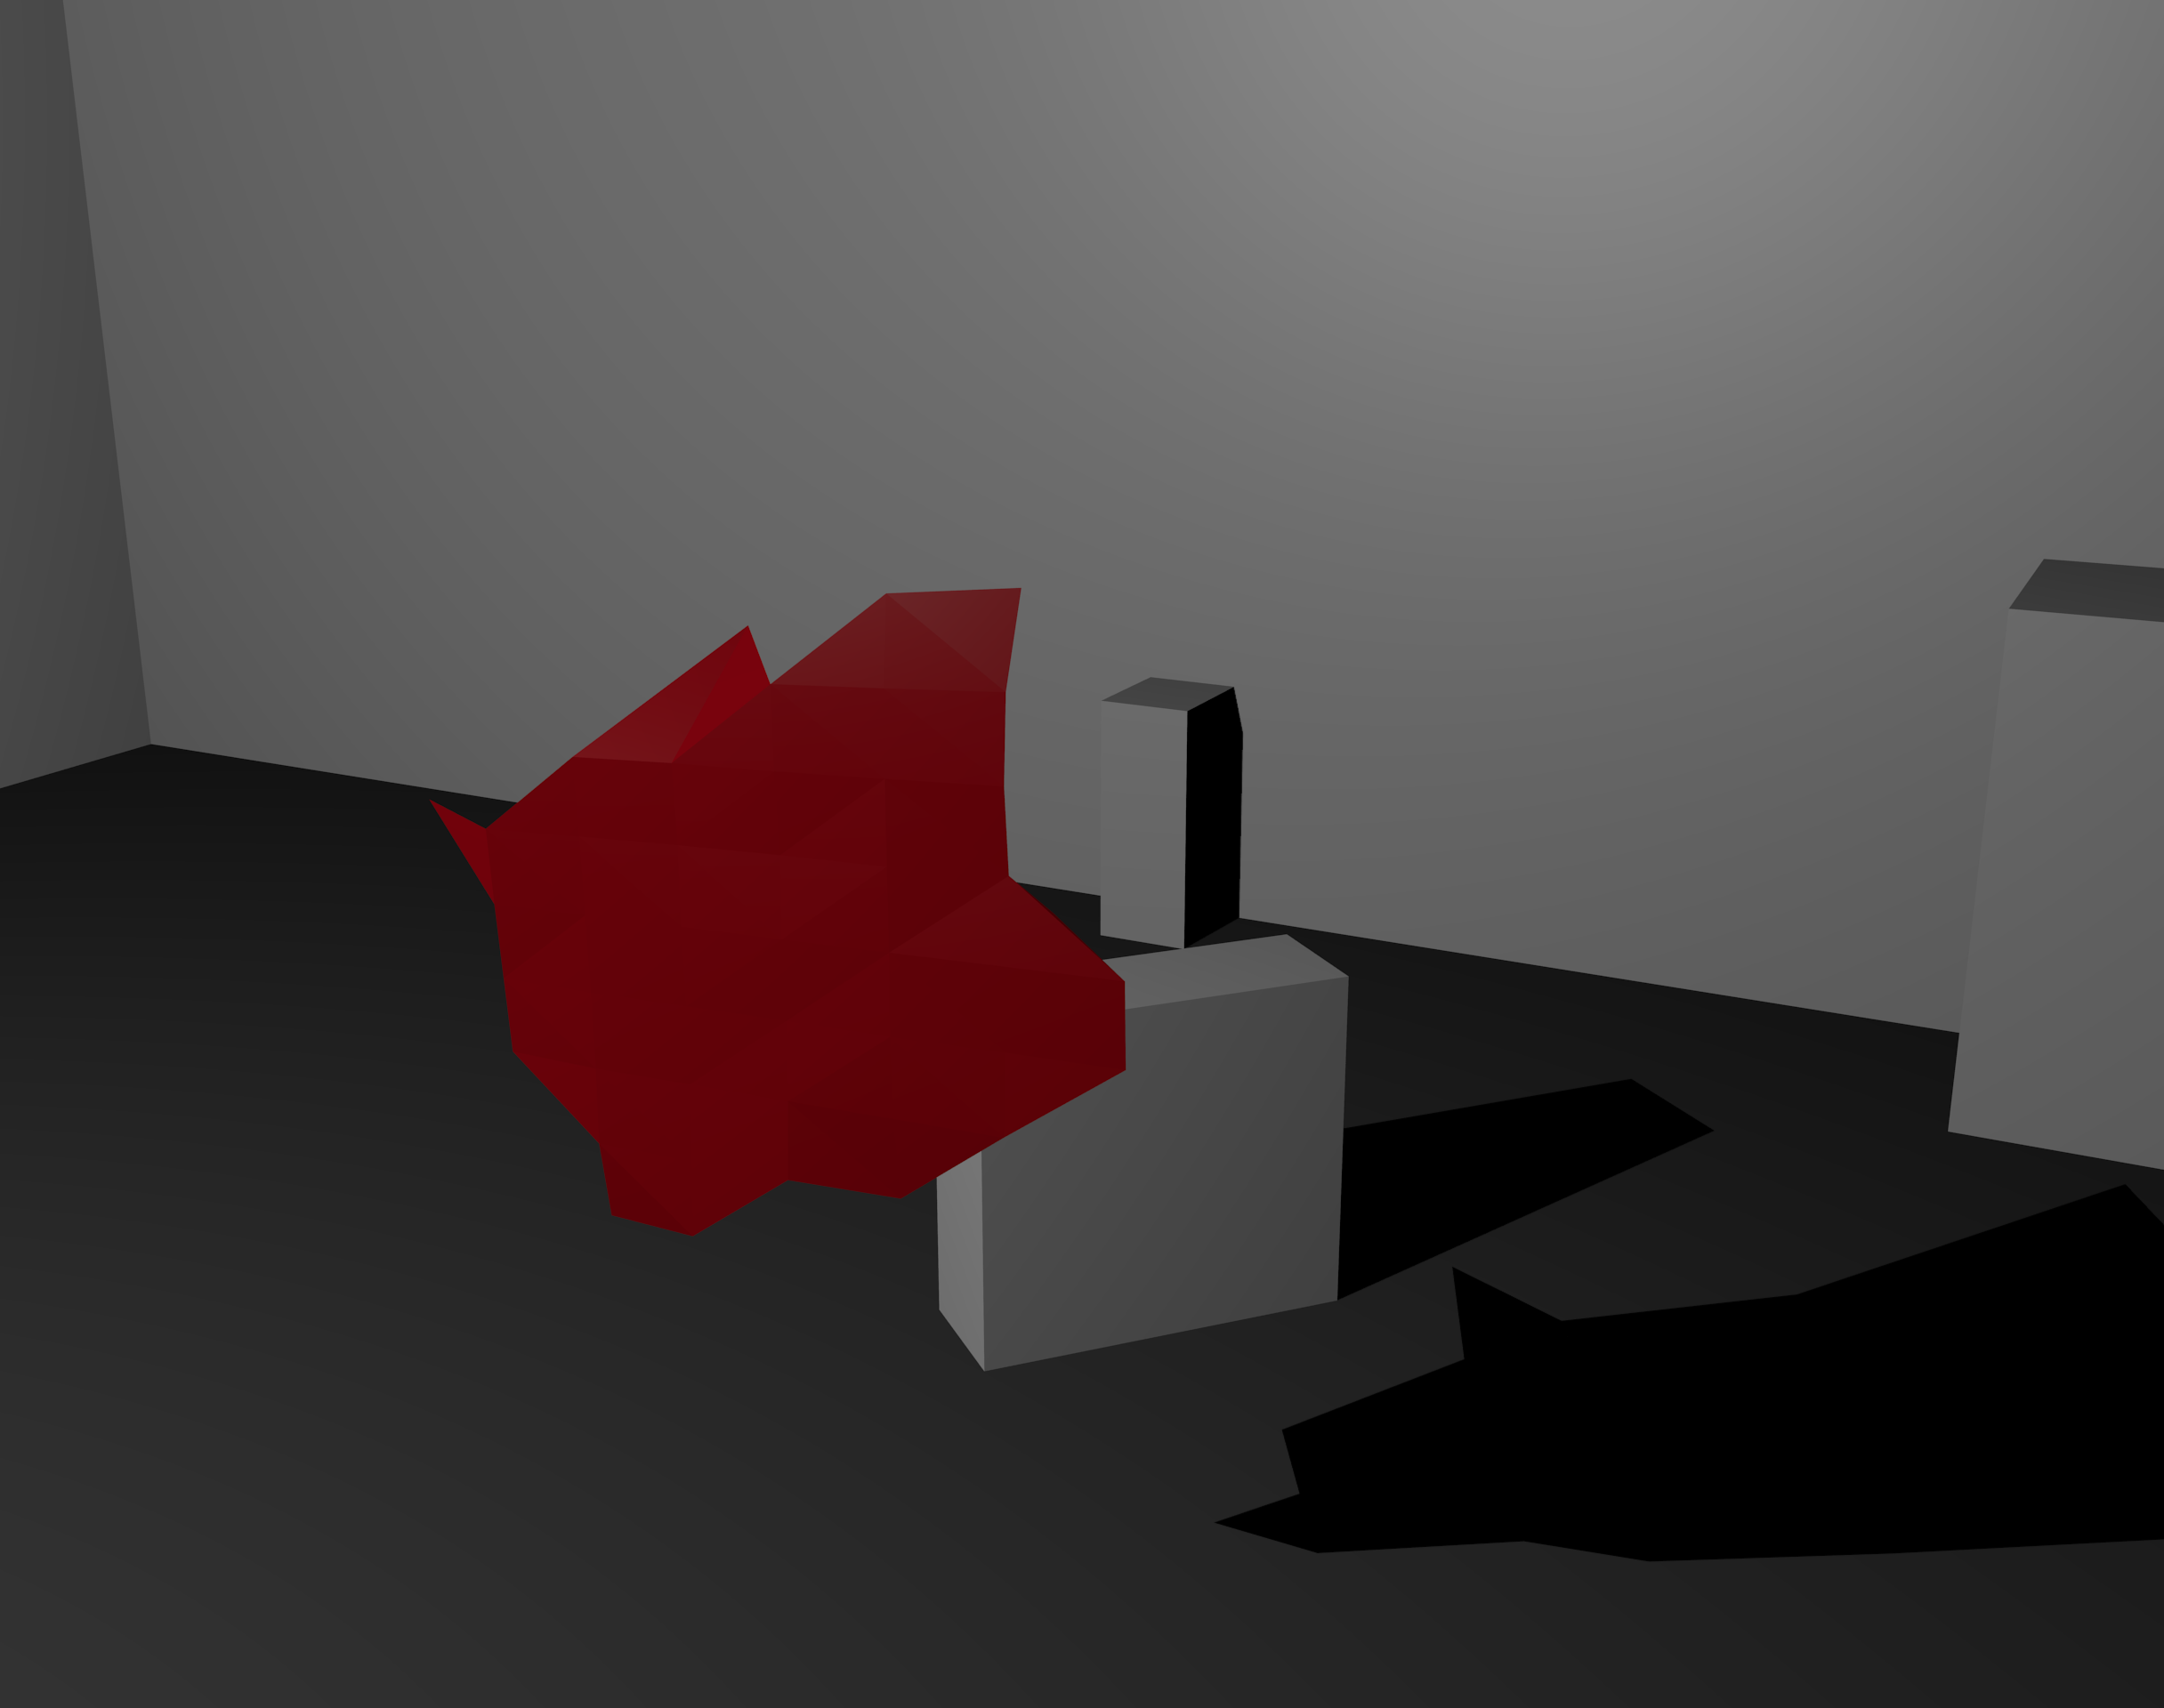
\includegraphics[width=5.0cm]{img/evaluation/test_set/rendered_obstacle}\\
		(c) Anzeigemodus Hindernis & (d) Hindernis Pointcloud als Mesh
		\end{tabular}
		\caption{Abbildungen (a) - (c) zeigen die sichtbaren Bilder während der Testaufnahme. (c) zeigt eine als Mesh gerenderte Pointcloud}
		\label{fig:test_viewing}
	\end{figure}
   	% TODO hindernisform: was ist daran gut / schlecht vielleicht

	\noindent
	\textbf{Großes Hindernis:}\\ 
    \noindent
	Im ersten Test wurde das große Hindernis gewählt, dabei wurde mithilfe der dargestellten Hindernisse auf der Disparity Map überprüft ob sich die erkannten Hindernisse innerhalb des Gefahrenbereichs befinden. Um auch kritische Bereiche zu testen wurde das Hindernis zudem zu Teilen außerhalb dieser platziert. Aus den 12 aufgenommenen Bildern des Testsets ergaben sich die in Abbildung \ref{fig:eval_big} (a) sichtbaren Ergebnisse.\\

	\begin{figure}[h]
		\centering
		\begin{tabular}{cc}
		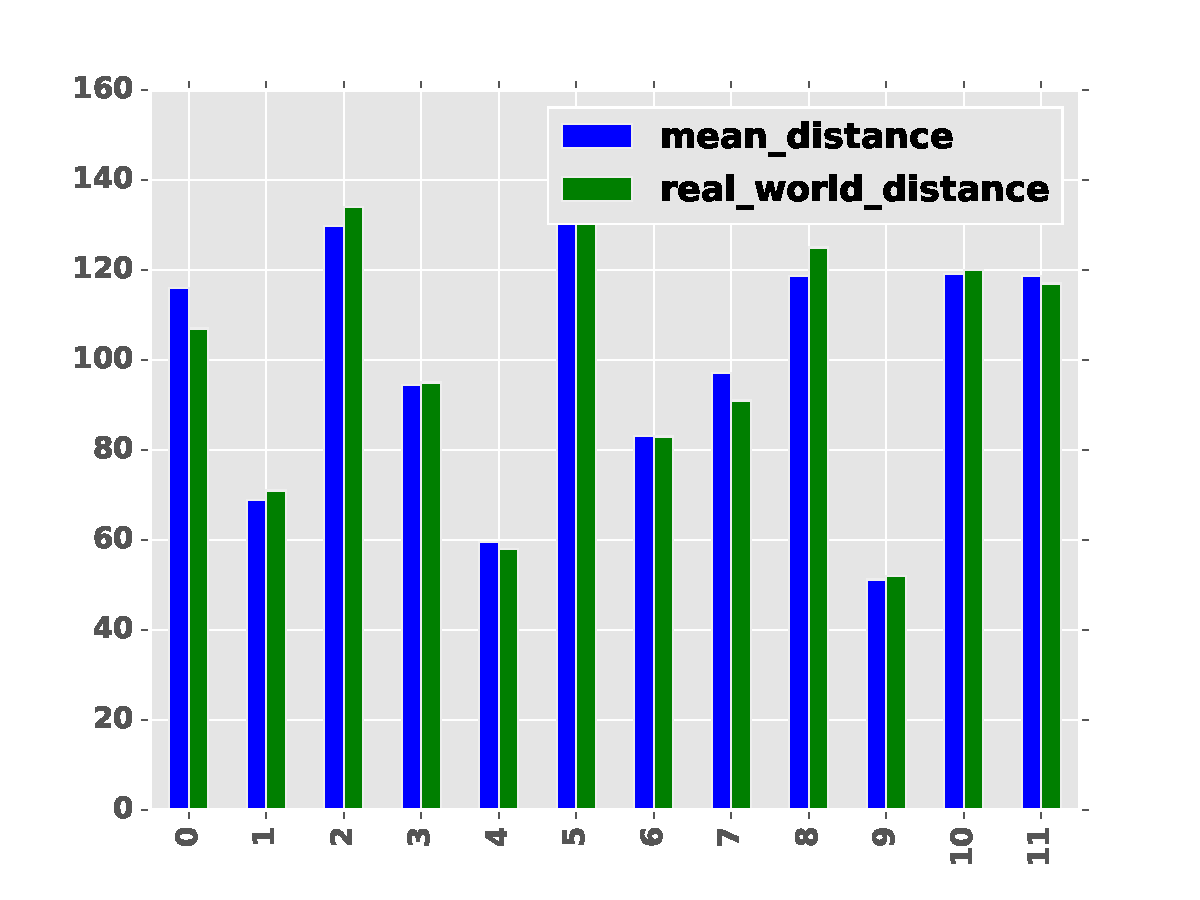
\includegraphics[width=7cm]{img/evaluation/sub_big_bar}&
		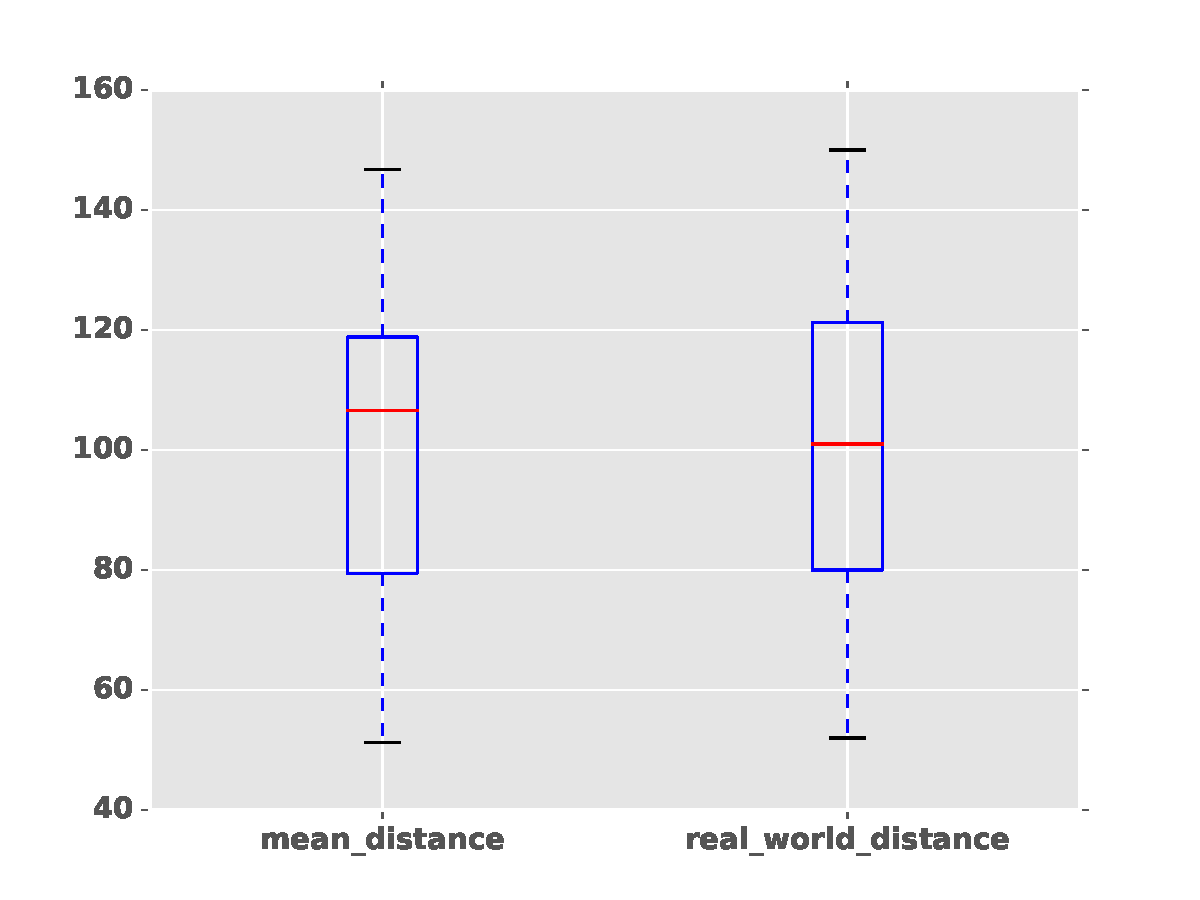
\includegraphics[width=7cm]{img/evaluation/sub_big_box}\\
		 (a) & (b)
		\end{tabular}
		\caption{}
	    \label{fig:eval_big}
	\end{figure}
	
	\noindent
	Wie aus dieser zu erkennen wurde in nahezu allen Frames das Hindernis richtig erkannt. Die berechneten Distanzen stimmen mit den real gemessenen überein. Minimale Abweichungen können in diesem Fall als Messungenauigkeit ignoriert werden, da der Mittelpunkt zwischen der minimalen und maximalen Objektdistanz kein statischer Punkt ist. Es wurden zwar alle Hindernisse erkannt, jedoch nicht der gesamte Bereich den sie umfasst haben. Wie Abbildung \ref{fig:eval_big_fails} zeigt wurden der obere und untere Bereich des Hindernisses im 5. Frame nicht erkannt. Dies könnte einerseits aus der Rotation des Objektes resultieren, andererseits auch aus einer gewissen Biegung die das physische Objekt mit sich bringt.
	
	\begin{figure}[h]
		\centering
		\begin{tabular}{cc}
		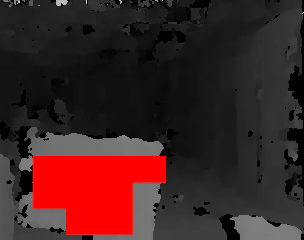
\includegraphics[width=5cm]{img/evaluation/_test_5_disparity}&
		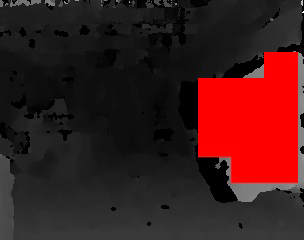
\includegraphics[width=5cm]{img/evaluation/_test_8_disparity}\\
		(a) Frame 5 &  (b) Frame 8
		\end{tabular}
		\caption{}
	    \label{fig:eval_big_fails}
	\end{figure}

	\noindent
	Auch im in Abbildung \ref{fig:eval_big} (b) abgebildeten Boxplot lässt sich erkennen, dass der Median beider gemessenen Distanzen, mit geringen Abweichungen, nahezu gleich ist. Auch die minimal und maximal Werte befinden sich, ebenfalls mit vernachlässigbarer Abweichungen auf derselben Gerade.\\

	\noindent
	\textbf{Mittleres Hindernis:}\\
	\begin{figure}[h]
		\centering
		\begin{tabular}{cc}
		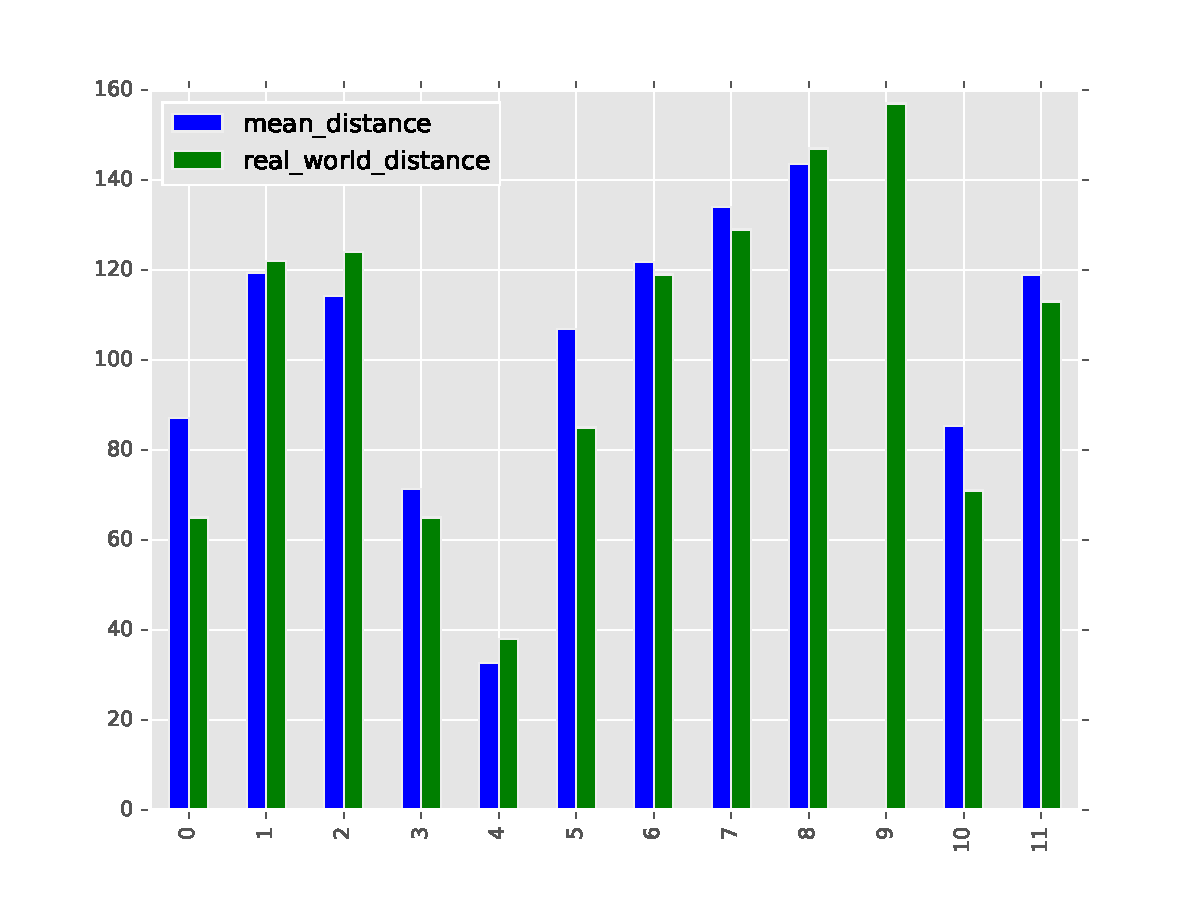
\includegraphics[width=7cm]{img/evaluation/sub_medium_bar}&
		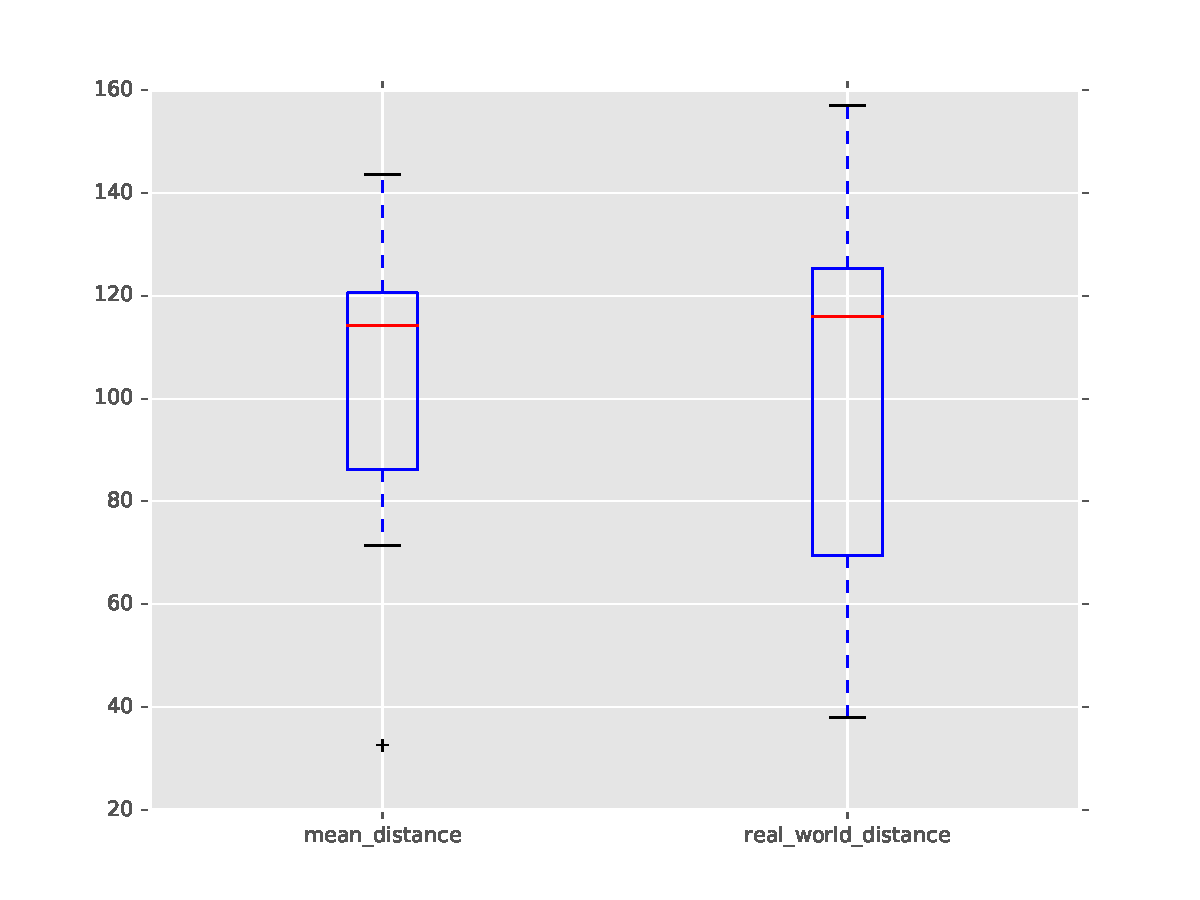
\includegraphics[width=7cm]{img/evaluation/sub_medium_box}\\
		(a) &  (b)
		\end{tabular}
	    \caption{}
	    \label{fig:eval_medium}
	\end{figure}
	
	\noindent
	Auch die Erkennung mittlerer Hindernisse durch den Algorithmus war in nahezu allen Fällen erfolgreich. Ein auffälliges Detail im Vergleich zu den Ergebnissen des großen Hindernisses ist die höhere Differenz aus berechneter und gemessener Distanz. Das getestete Objekt befand sich während der Tests an einem durchsichtigen Plexiglas Stab. Dieser ist teilweise auch als Hindernis erkannt worden. Im Fall von Frame 8 umfasst das Objekt insgesamt 17 Subimages in denen es erkannt wurde. Als Resultat des Stabes wurden jedoch noch 2 weitere erkannt. Frame 1 weist zwar keine große Abweichung zwischen der berechneten und realen Distanz auf, jedoch wird das Objekt zu teilen nicht erkannt. Bei einer Distanz von $120\ cm$ ist eine Erkennung dieser Hindernisgröße in nur 2 Subimages ungewöhnlich. Dies könnte zum Teil aus der verwendeten Blockgröße resultieren.
	
	% TODO bilder des aktuellen sets nehmen
	\begin{figure}[h]
		\centering
		\begin{tabular}{cc}
		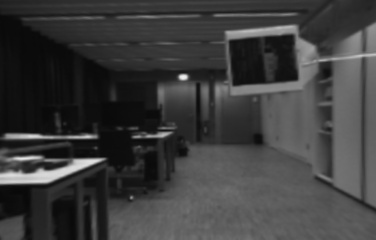
\includegraphics[width=5cm]{img/evaluation/medium_0_left}&
		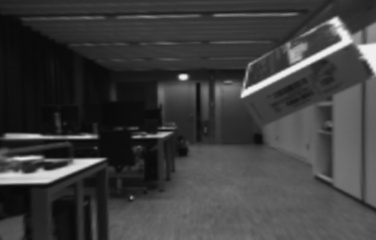
\includegraphics[width=5cm]{img/evaluation/medium_3_left}\\
		(a) Frame 0 &  (b) Frame 3
		\end{tabular}
		\caption{}
		\label{fig:eval_medium_fails}
	\end{figure}
	
	\noindent
	Selbiges Resultat lässt sich in den Frames 2, 6 und 7 erkennen. In Frame 9 dagegen konnte kein Hindernis erkannt werde, da sich das Objekt an der Grenze der Gefahrenzone befunden hat und demnach die Abweichung der Disparität zu keiner Erkennung führen konnte. Eben diese Ergebnisse sind auch in Abbildung \ref{fig:eval_medium} (sb) sichtbar, das Maximum der realen Distanz resultiert dabei aus dem nicht erkannten Hindernis in Frame 9.\\
	
	\noindent
	\textbf{Winziges Hindernis:}\\
	\begin{figure}[h]
		\centering
		\begin{tabular}{cc}
		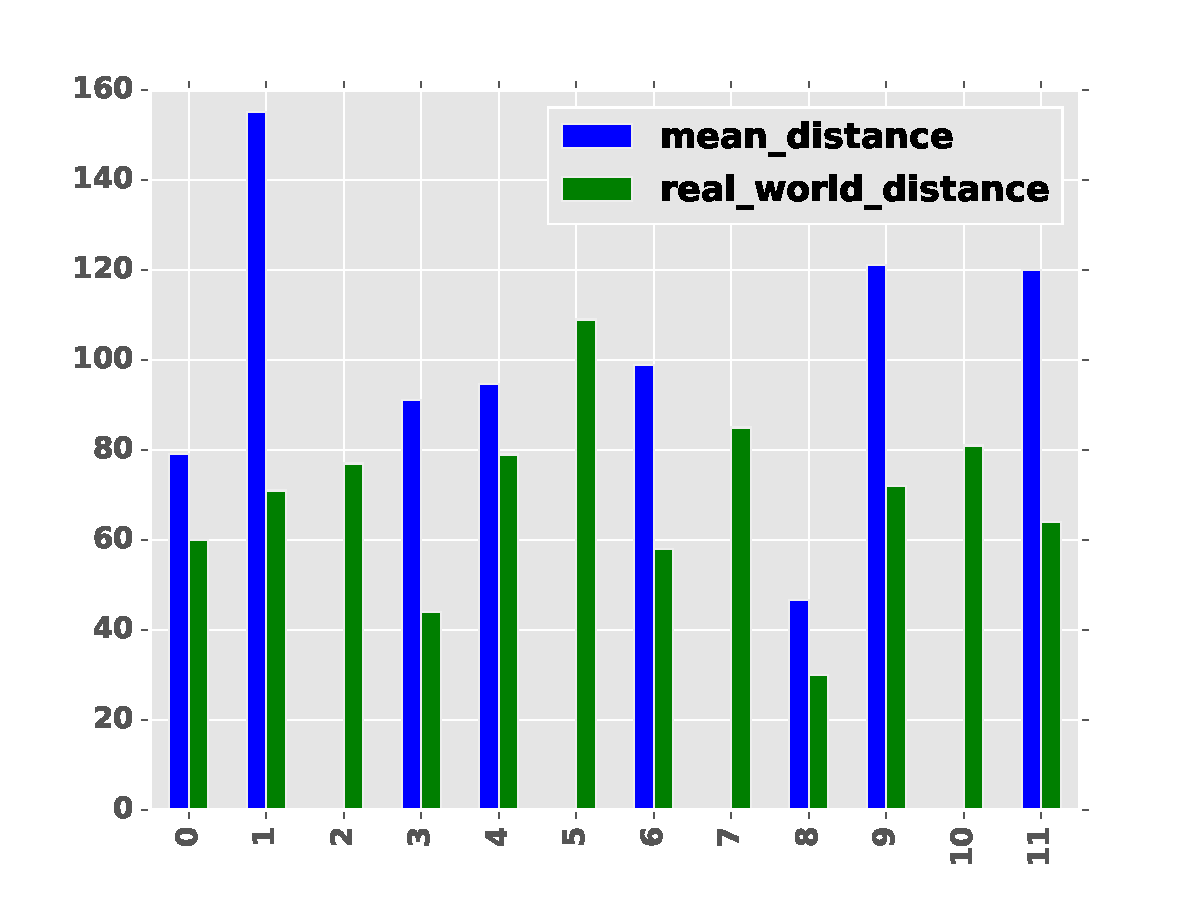
\includegraphics[width=7cm]{img/evaluation/sub_tiny_bar}&
		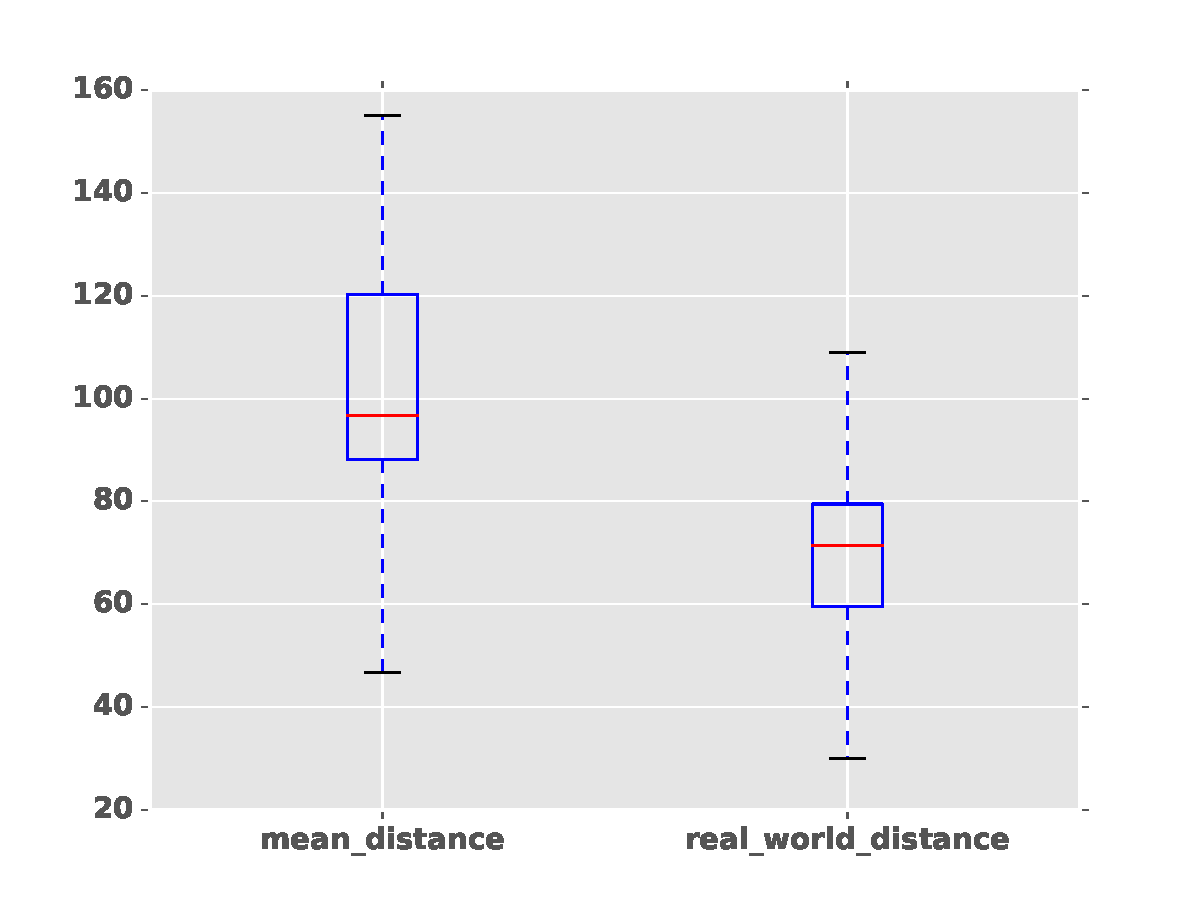
\includegraphics[width=7cm]{img/evaluation/sub_tiny_box}\\
		(a)	& (b)
		\end{tabular}
	    \caption{}
	    \label{fig:eval_tiny}
	\end{figure}
	
	\noindent
	Die Erkennung winziger Hindernisse gestaltet sich aufgrund diverser Faktoren schwer. Ein limitierender Faktor ist die Fläche, ist ein einzeles Hindernis so klein, dass es während der Berechnung des Medians aufgrund der umliegenden Disparitäten untergeht, so kann auch kein Hindernis erkannt werden. Dies macht sich in vielen der getesteten Bildern bemerkbar. In den Frames 2, 5, 7 und 10 wurde das Hindernis nicht erkannt, da es sich entweder an einer Kreuzung verschiedener Subimages befand, oder die verwendete Blockgröße nicht ausreicht, dadurch wird der Median aller Teilmatrizen nicht signifikant beeinflusst. Auch der Stab wurde in den Frames 3, 6 sowie 8 als zusätzliches Hindernis erkannt. Dies ist ein Resultat der relativ geringen Distanz zu den Kameras. Die hohen Entfernungsdifferenzen resultieren in diesen Fällen wiederum aus der großen Entfernung der Hindernisse zum Hintergrund sowie dem auftretenden Schatten welcher durch die Baseline zu begründen ist. Auch der in Abbildung \ref{fig:eval_tiny} (b) dargestellte Boxplot zeigt, das signifikant größere Distanzen erkannt wurden als sie in den realen Messungen vorkommen.

% ---------------------- section -----------------------
\section{Evaluierung Samplepoint Detection}
\label{sec:evaluierung_samplepoint}

	\noindent
	Durch die wesentlich höhere Anzahl an betrachteten Bereichen innerhalb der Disparity Map ist anzunehmen, dass die Erkennung kleiner Hindernisse eine höhere Erfolgswahrscheinlichkeit verspricht. Im Rahmen dieses Abschnittes wird die Samplepoint Detection getestet. Dies geschieht nach dem in \ref{sec:evaluierung_subimage} bereits beschriebenen Schema.\\

	\noindent
	\textbf{Großes Hindernis:}\\
	Die Erkennung großer Objekte der Samplepoint Detection weist nahezu keine Fehler auf. Abbildung \ref{fig:sample_eval_big} zeigt das jede der 12 Ausrichtungen des Objektes erkannt wurden. Die dabei auftretenden Differenzen zwischen der berechneten sowie gemessenen Distanz sind auf Messungenauigkeiten zurückzuführen. Auch in Grenzbereichen nahe dem Rand des Gefahrenbereichs wurden die Hindernisse erkannt. 
	
    \begin{figure}[h]
		\centering
		\begin{tabular}{cc}
		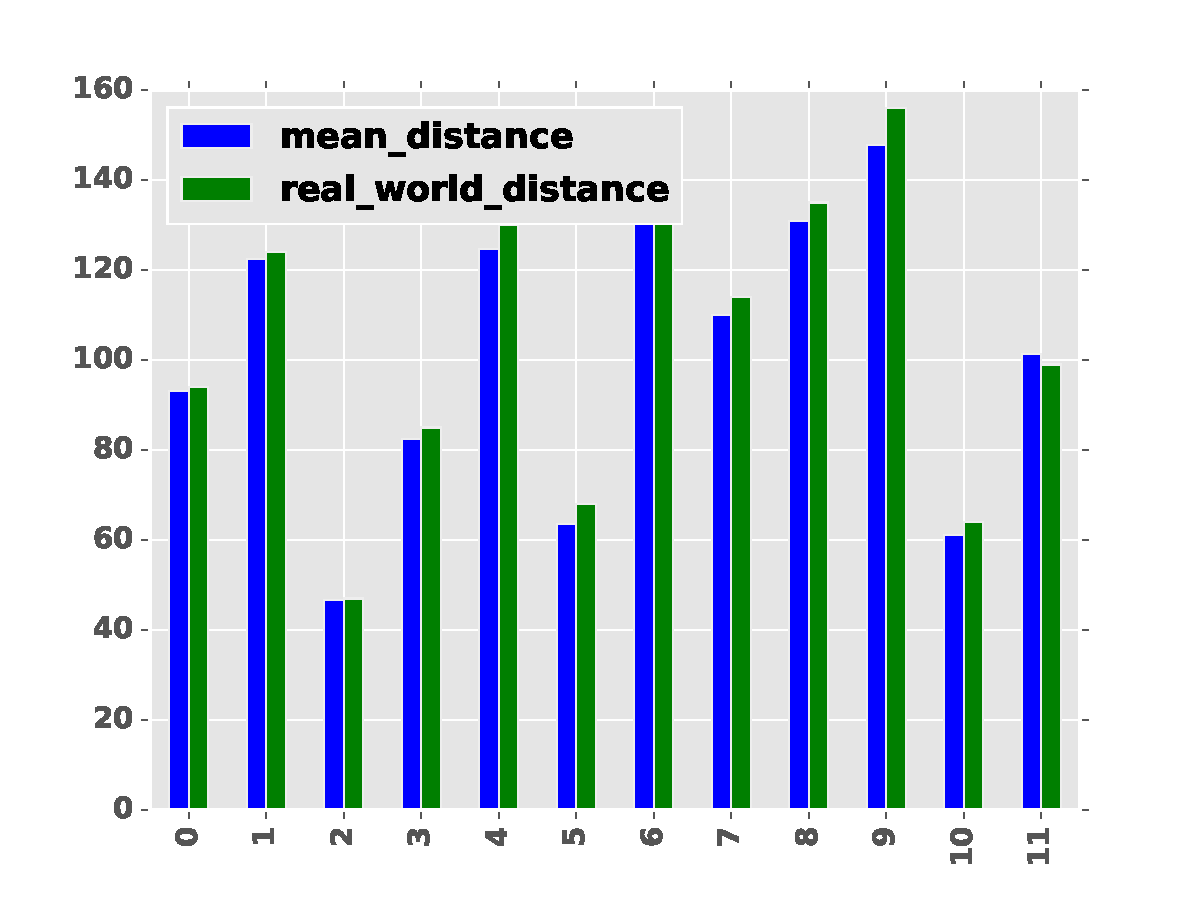
\includegraphics[width=7cm]{img/evaluation/sample_big_bar}&
		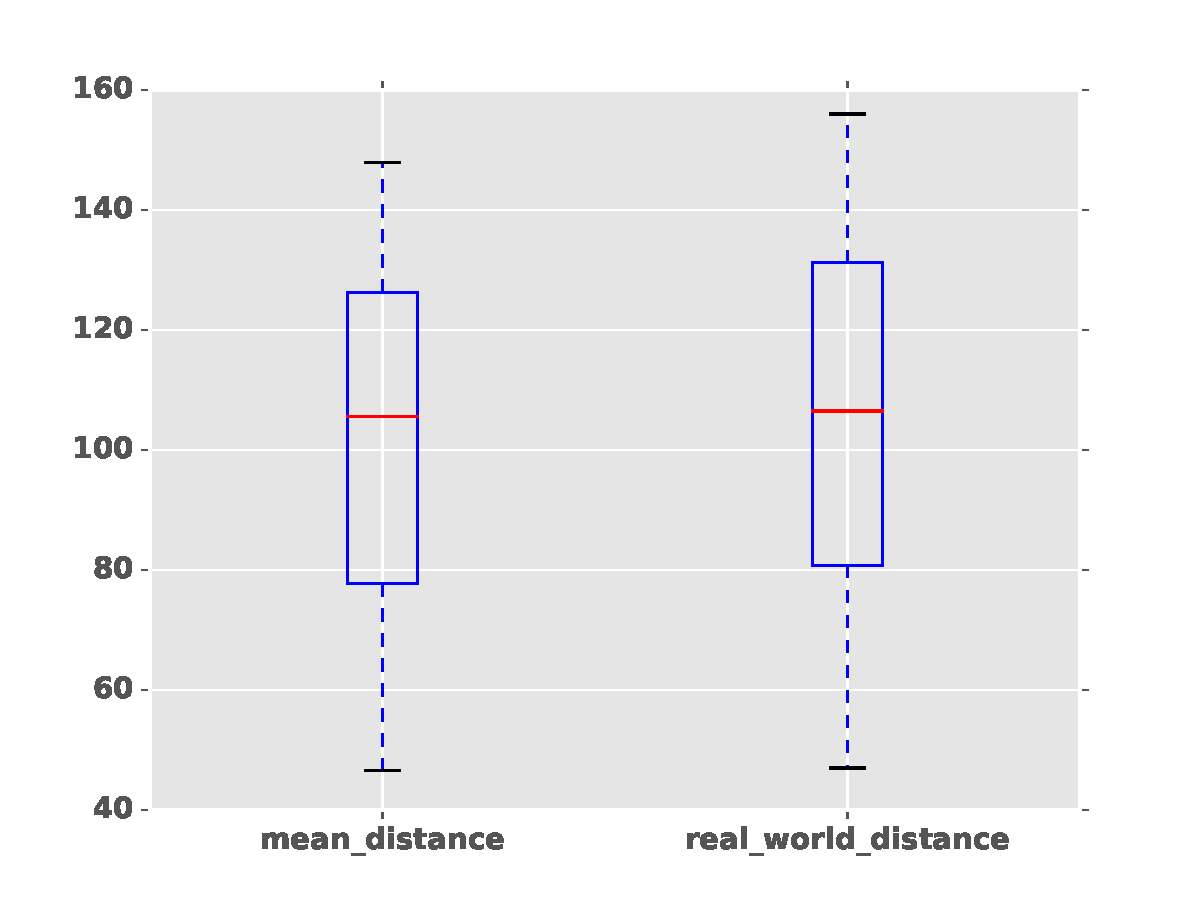
\includegraphics[width=7cm]{img/evaluation/sample_big_box}\\
		 (a) & (b)
		\end{tabular}
		\caption{}
	    \label{fig:sample_eval_big}
	\end{figure}

	\noindent
	\textbf{Mittleres Hindernis:}\\

	\begin{figure}[h]
		\centering
		\begin{tabular}{cc}
		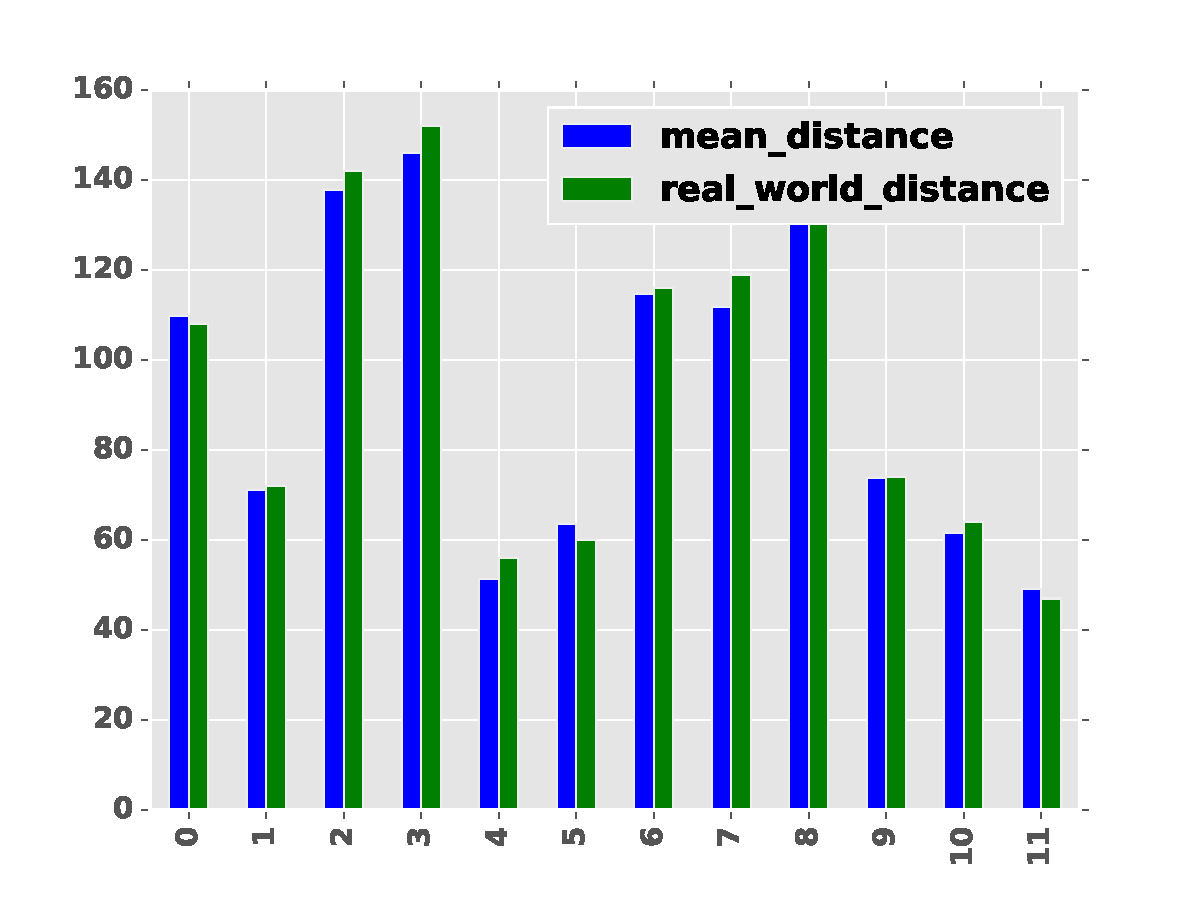
\includegraphics[width=7cm]{img/evaluation/sample_medium_bar}&
		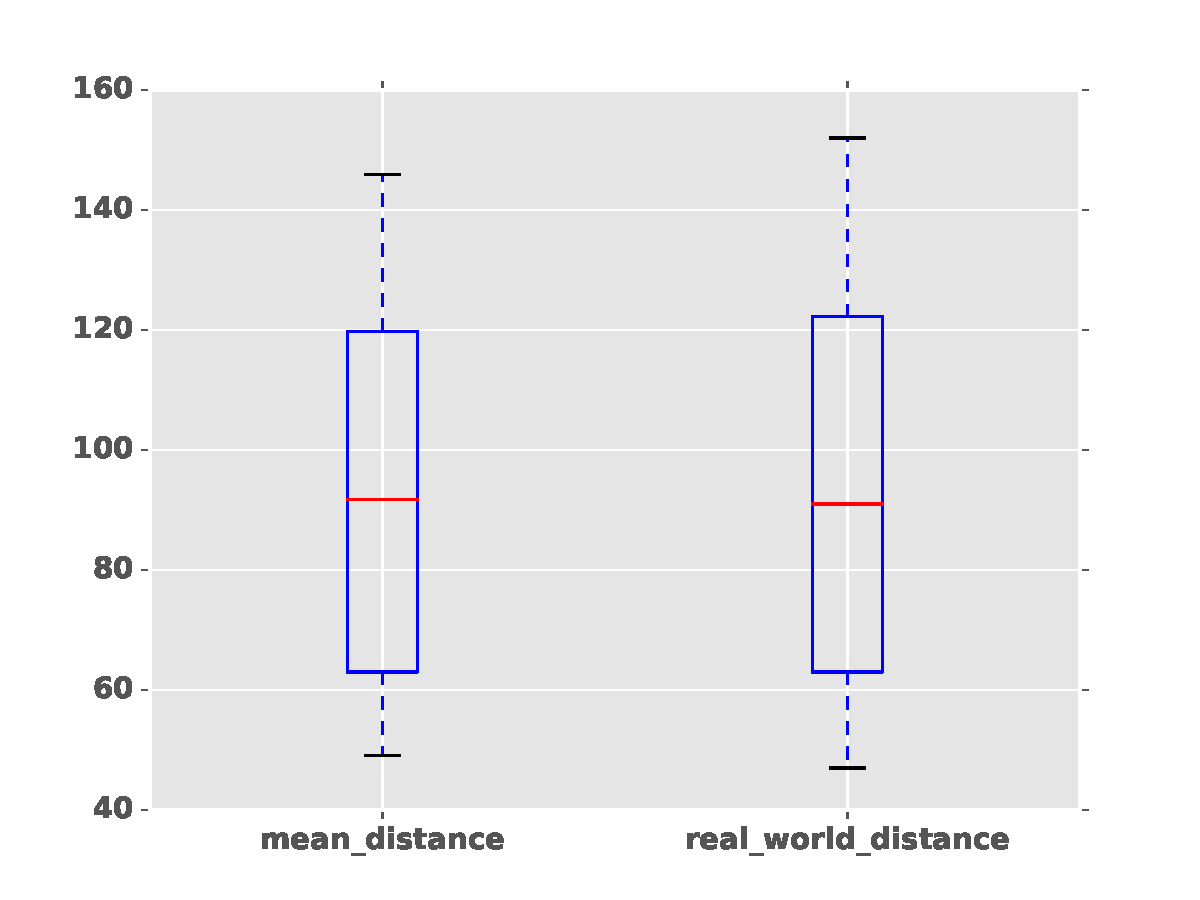
\includegraphics[width=7cm]{img/evaluation/sample_medium_box}\\
		 (a) & (b)
		\end{tabular}
		\caption{}
	    \label{fig:sample_eval_medium}
	\end{figure}

	\noindent
	Auch die Erkennung mittlerer Hindernisse erfolgte in allen Frames ohne signifikante Probleme (siehe Abbildung \ref{fig:sample_eval_medium}). Bereiche in denen aufgrund fehlender Textur keine Korrespondenz zugeordnet werden konnte wurden aufgrund der hohen Dichte der Samplepoints trotzdem erkannt. Wie Abbildungen \ref{fig:sample_eval_medium_fails} (a) und (b) zeigen wurden nicht gematchte Bereiche auch nicht als Hindernis erkannt, die umliegenden Texturierten Bereiche überwiegen diese doch und sorgen daher für eine robuste Detektion. 

	\begin{figure}[h]
		\centering
		\begin{tabular}{cc}
		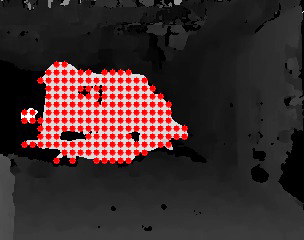
\includegraphics[width=5cm]{img/evaluation/sample_tiny_test_5_disparity}&
		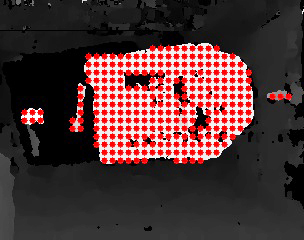
\includegraphics[width=5cm]{img/evaluation/sample_tiny_test_11_disparity}\\
		(a) Frame 5 &  (b) Frame 11
		\end{tabular}
		\caption{}
		\label{fig:sample_eval_medium_fails}
	\end{figure}
	
	\noindent
	Die bereits beschriebene hohe Dichte der Samplepoints und deren geringe Größe hilft auch hier wieder den Stab als Hindernis zu erkennen (siehe Abbildung \ref{fig:sample_eval_medium_fails} (b))


	\noindent
	\textbf{Winziges Hindernis:}\\


	\begin{figure}[h]
		\centering
		\begin{tabular}{cc}
		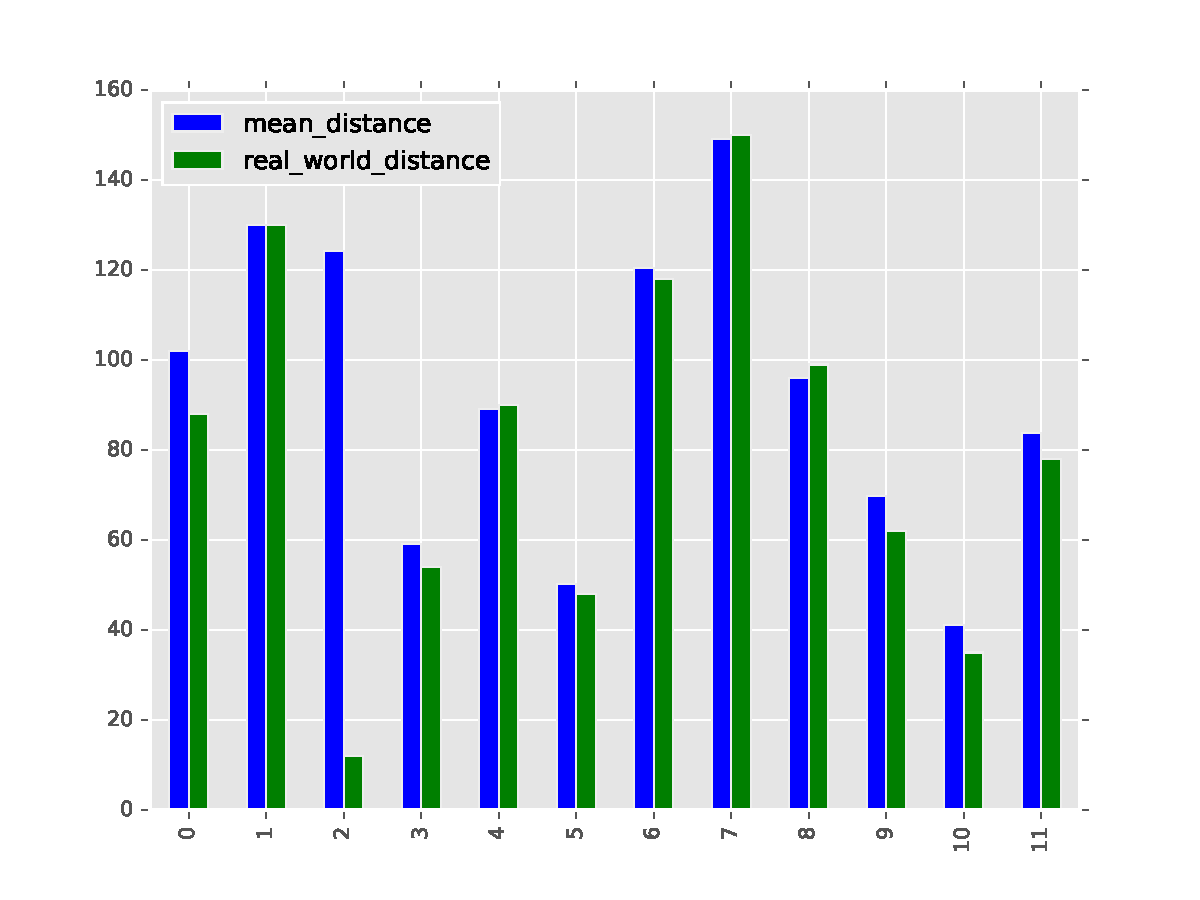
\includegraphics[width=7cm]{img/evaluation/sample_tiny_bar}&
		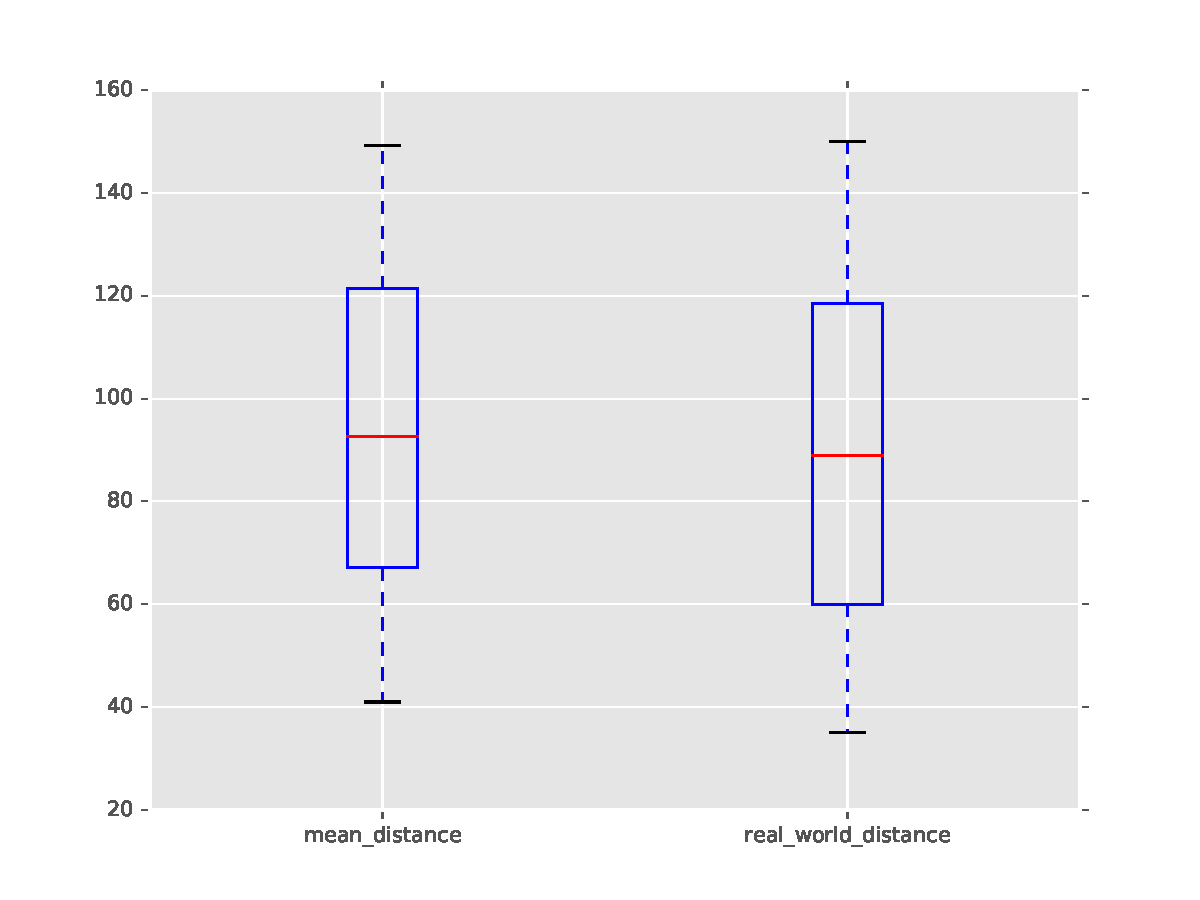
\includegraphics[width=7cm]{img/evaluation/sample_tiny_box}\\
		 (a) & (b)
		\end{tabular}
		\caption{}
	    \label{fig:sample_eval_tiny}
	\end{figure}

